\documentclass[../main/main.tex]{subfiles}

\raggedbottom

\makeatletter
\renewcommand{\@chapapp}{Chimie -- chapitre}
\makeatother

\begin{document}
\setcounter{chapter}{0}

\chapter{Introduction \`a la chimie}

La chimie se concentre à décrire la matière et ses transformations, mais
lesquelles~? Comment caractérise-t-on physiquement et mathématiquement les états
et leurs transformations~?

\section{Vocabulaire général}
\subsection{Atomes et molécules}
Ce sont les briques de ce qui constitue la matière à l'échelle nanoscopique.

\subsubsection{Les atomes}
\begin{tcbraster}[raster columns=2, raster equal height=rows]
    
    \begin{defi}[label=def:atome]{Atome}
        L'atome est un constituant \textbf{neutre} de la matière, comportant un
        noyau central entouré d'un nuage électronique. Le noyau est composé de
        particules nommées \textbf{nucléons} dont il existe deux sortes~:
        \begin{itemize}
            \item \textbf{les protons}, de charge $+e$ et de masse $m_p =
                \SI{1.673e-27}{kg}$~;
            \item \textbf{les neutrons}, de charge nulle et de masse $m_n =
                \SI{1.675e-27}{kg}$.
        \end{itemize}
        % La taille du noyau d'un atome est de l'ordre de \SI{e-15}{m}, soit
        % \SI{1}{fm} (femtomètre).
        Le nuage électronique est composé
        \begin{itemize}
            \item d'\textbf{électrons}, de charge $-e$ et de masse $m_e =
                \SI{9.1e-31}{kg}$.
        \end{itemize}
        % Un atome avec son nuage électronique fait une taille de l'ordre de
        % \SI{e-10}{m} soit \SI{0.1}{nm}.
    \end{defi}
    \begin{defi}[label=def:numéroatomique]{numéro atomique et nombre de nucléons}
        Pour représenter un atome de façon symbolique, on utilise son symbole
        chimique, noté X ici dans le cas général, accompagné de deux nombres~:
        \begin{itemize}
            \item Son \textbf{numéro atomique}, soit le nombre de \textbf{protons}
                contenus dans le noyau. Il est noté $Z$, et définit l'élément
                chimique~;
            \item Le nombre de \textbf{nucléons}, également appelé le \textbf{nombre
                de masse}, noté $A$. 
        \end{itemize}
        On écrit alors

        \centers{$\prescript{A}{Z}{\mathrm{X}}$}
    \end{defi}

    \begin{rema}[label=rema:atomeneutre]{nombre d'électrons et de masse}
        Un atome étant neutre, indiquer son nombre de protons suffit~: le nuage
        électronique sera constitué d'autant d'électrons que de protons dans le
        noyau. De plus, les électrons étant $\approx 1000$ fois plus légers que les
        nucléons, on les néglige souvent dans le calcul de la masse d'un atome, d'où
        l'appellation \textbf{nombre de masse} pour $A$.
    \end{rema}
    \begin{exem}[label=exem:atomes]{}
        \begin{itemize}
            \item L'atome de bore $ \prescript{10}{5}{\mathrm{B}}$ possède 5
                protons, donc 5 électrons, et $10-5=5$ neutrons~;
            \item L'atome d'oxygène $\prescript{16}{8}{\mathrm{O}}$ possède 8
                protons et $16-8=8$ neutrons~;
            \item L'atome de fer $ \prescript{56}{26}{\mathrm{Fe}}$ possède 26
                protons et $56-26 = 30$ neutrons;
            \item L'atome de plomb $\prescript{208}{82}{\mathrm{Pb}}$ possède 82
                protons et $208 - 82 = 126$ neutrons.
        \end{itemize}
    \end{exem}
\end{tcbraster}

% \vspace{-15pt}
\subsubsection{Les ions}

\begin{tcbraster}[raster columns=2, raster equal height=rows]
    \begin{defi}[label=def:ion]{Ion}
        Un \textbf{ion} est un atome qui a \textbf{perdu ou gagné un ou plusieurs
        électrons}. On indique leur charge en haut à droite de l'élément chimique.
        On a alors deux types d'ions~:
        \begin{itemize}
            \item les \textbf{cations} qui sont chargés \textbf{positivement},
                c'est-à-dire que c'est un atome qui a \textbf{perdu} un ou plusieurs
                électrons~;
            \item les \textbf{anions} qui sont chargés \textbf{négativement},
                c'est-à-dire que c'est un atome qui a \textbf{gagné} un ou plusieurs
                électrons.
        \end{itemize}
    \end{defi}
    \begin{exem}[label=exem:ion]{}
        \begin{itemize}
            \item L'ion sodium Na$\plus{}$ possède 11 protons, et donc 10 électrons.  
            \item L'ion chlorure Cl$\moin{}$ possède 17 protons et donc 18
                électrons. 
        \end{itemize}
        \begin{itemize}
            \item L'ion fer Fe$\plus{2}$ possède 26 protons, 24 électrons. 
            \item L'ion oxyde O$\moin{2}$ possède 16 protons et 18 électrons.
        \end{itemize}
    \end{exem}
\end{tcbraster}

\subsubsection{Les molécules}
\begin{tcbraster}[raster columns=2, raster equal height=rows]
    \begin{defi}[label=def:molécules]{molécules}
        Les molécules ou les ions polyatomiques sont des assemblages d'atomes
        liés entre eux grâce à des liaisons chimiques. Ces liaisons chimiques se
        créent dès que l'énergie des atomes «~liés~» est plus faible que la
        somme des énergies des atomes séparés. Ainsi, des atomes engagés dans
        une molécule sont plus stables que s'ils étaient seuls, d'où l'existence
        des molécules.
    \end{defi}
    \begin{exem}[label=exem:molécules]{molécules}
        \begin{itemize}
            \item Le méthane est l'assemblage d'un atome de carbone et de 4
                atomes d'hydrogène~: on l'écrit CH$_4$~;
            \item Le dioxygène est la molécule composée de deux atomes d'oxygène
                liés entre eux~: on l'écrit O$_2$.
        \end{itemize}
    \end{exem}
\end{tcbraster}

\subsection{États de la matière}
\begin{defi}[label=def:etat]{états ou phases de la matière}
    La matière est naturellement présente sous 3 formes, que l'on
    appelle \textbf{états} ou \textbf{phases}~:
    \begin{itemize}
        \item \textbf{Solide}~: un solide a une forme propre, un volume
            propre, et peut être ordonné (cristal) ou non (verre)~;
        \item \textbf{Liquide}~: un liquide est dense mais désordonné
            (entités chimiques déplaçables les unes par rapport aux autres),
            et prend la forme de son contenant~;
        \item \textbf{Gazeux}~: un gaz est très peu dense et désordonné, et
            occupe \textit{tout le volume accessible}~;
    \end{itemize}
\end{defi}

\begin{tcbraster}[raster columns=2, raster equal height=rows]
    \begin{defi}[label=def:solu]{solutés et solutions}
        On trouve également partout des \textbf{solutés}, c'est-à-dire de la
        matière dans une solution liquide. Une \textbf{solution} est obtenue par
        dissolution d'un composé chimique dans un liquide nommé
        \textbf{solvant}. Une fois dissoute, l'espèce chimique est nommée le
        \textbf{soluté}.\bigbreak

        Avant dissolution, l'espèce en question peut être un solide, un liquide
        ou un gaz. Elle peut être constituée d'ions ou de molécules. Lorsque le
        solvant est de l'eau, on parle de \textbf{solution aqueuse}.
    \end{defi}
    \begin{exem}[label=exem:solution]{solutions}
        On peut dissoudre~: 
        \begin{itemize}
            \item De l'acide chlorhydrique gazeux dans de l'eau~;
            \item De l'éthanol liquide dans de l'eau~;
            \item Du sel (NaCl, solide ionique) dans de l'eau (les ions Na$^+$ et
                Cl$^-$ sont alors dissociés)~;
            \item Du sucre (solide moléculaire) dans de l'eau~;
            \item Du diiode dans de l'acétone…
        \end{itemize}
    \end{exem}
\end{tcbraster}

\begin{tcbraster}[raster columns=2, raster equal height=rows]
    \begin{nota}[label=nota:état]{état de la matière}
        Les états des composés chimiques sont indiqués généralement en indice et
        toujours entre parenthèses. On note~:
        \begin{itemize}
            \item (g) pour un gaz~;
            \item (liq) ou (l) pour un liquide~;
            \item (s) pour un solide~;
            \item (aq) pour un soluté.
        \end{itemize}
    \end{nota}
    \begin{exem}[label=exem:notationétat]{notations}
        \begin{itemize}
            \item Par exemple O$_{2}$$\gaz$~;
            \item Par exemple H$_2$O$_{\rm (liq)}$~;
            \item Par exemple Fe$\sol$~;
            \item Par exemple Na$\aqu\plus{}$.
        \end{itemize}
        La dissolution du sel NaCl$\sol$ donne une solution composée  d'eau liquide
        H$_2$O$\liq$, d'ion sodium Na$\aqu\plus{}$ et d'ion chlorure
        Cl$\aqu\moin{}$.
    \end{exem}
\end{tcbraster}

% \subsection{Systèmes physico-chimiques}
% 

\subsection{Transformations de la matière}

La matière peut subir des transformations de différentes natures, qui sont
traduites par des \textbf{équations-bilan}.

\begin{tcbraster}[raster columns=2, raster equal height=rows]
    \begin{defi}[label=def:eqbil]{équation bilan}
        L'équation-bilan d'une réaction indique les éléments de
        départ (\textbf{réactifs}) et les éléments de fin (\textbf{produits}),
        leur état physique si nécessaire ainsi que les proportions dans
        lesquelles ils apparaissent. Le signe entre les réactifs et produits
        peut être une flèche simple de gauche à droite ou de droite à gauche,
        les deux flèches ensemble ou un signe égal, selon les propriétés de la
        réaction.
    \end{defi}
    \begin{rema}[label=rema:eqbil]{équation bilan}
        \begin{itemize}
            \item L'équation-bilan ne fait apparaître que les espèces qui se
                transforment, pas les espèces nécessaires à la réaction
                mais dont la quantité ne varie pas (par
                exemple l'eau lors d'une dissolution).
            \item Après l'écriture d'une réaction, il faut \textbf{toujours}
                vérifier qu'elle est équilibrée, tant en \textbf{nombre d'atome}
                qu'en \textbf{nombre de charges}
        \end{itemize}
    \end{rema}
\end{tcbraster}

\subsubsection{Transformations nucléaires}

\begin{tcbraster}[raster columns=2, raster equal height=rows]
    \begin{defi}[label=def:transnuc]{transformations nucléaires}
        Au cours d'une \textbf{transformation nucléaire}, un ou plusieurs
        \textbf{noyaux} atomiques sont modifiés.
    \end{defi}
    \begin{exem}[label=exem:transnuc]{transformation nucléaire}
        Lors de la désintégration radioactive (type $\alpha$) de l'uranium 238,
        le noyau d'uranium perd 4 nucléons, 2 protons et 2 neutrons.
        \begin{equation*}
            \prescript{238}{92}{\mathrm{U}}
            \longrightarrow 
            \prescript{234}{90}{\mathrm{Th}} + \prescript{4}{2}{\mathrm{He}}
        \end{equation*}
    \end{exem}
\end{tcbraster}

\subsubsection{Transformations physiques}

\begin{tcbraster}[raster columns=2, raster equal height=rows]
    \begin{defi}[label=def:transnuc]{transformations physiques}

        Au cours d'une \textbf{transformation physique}, unes espèce chimique
        subit une \textbf{transition de phase} (i.e.\ un changement d'état de
        matière) \textbf{sans modification du noyau ou des liaisons entre
        atomes}.
    \end{defi}
    \begin{exem}[label=exem:transnuc]{transformation physique}
        \begin{center}
            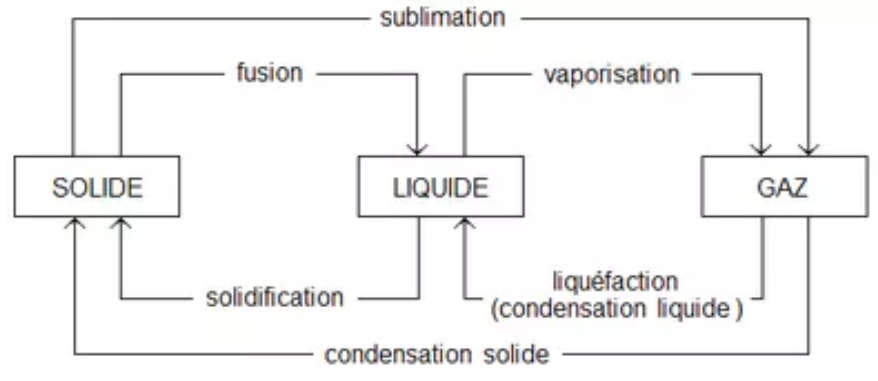
\includegraphics[width=\linewidth]{trans_phase}
        \end{center}
        Sublimation du dioxyde de carbone solide
        \[ \mathrm{CO}_2{}\sol
            \longrightarrow
        \mathrm{CO}_2{}\gaz\]
    \end{exem}
\end{tcbraster}

\subsubsection{Transformations chimiques}

\begin{tcbraster}[raster columns=2, raster equal height=rows]
    \begin{defi}[label=def:transnuc]{transformations chimiques}

        Au cours d'une \textbf{transformation chimique}, il y a réorganisation
        des atomes d'une ou plusieurs substances. On observe la formation et la
        rupture d'une ou plusieurs liaisons. Les coefficients devant les espèces
        sont appelés \textbf{nombres stœchiométriques}.
    \end{defi}
    \begin{exem}[label=exem:transnuc]{transformation chimique}
        Combustion du méthane~:
        \begin{equation*}
            \mathrm{CH}_4{}\gaz + 2\mathrm{O}_2{}\gaz
            =
            \mathrm{CO}_2{}\gaz + 2\mathrm{H}_2\mathrm{O}\gaz
        \end{equation*}
    \end{exem}
\end{tcbraster}

\section{Quantité de matière}
\subsection{La mole}

Les molécules réagissent dans des proportions bien précises, notamment pour
conserver le nombre d'atome. Il serait donc utile de déterminer le nombre de
molécules ou d'atomes qui peuvent réagir au sein d'un échantillon. On se rend
vite compte que les nombres sont très grands et difficiles d'appréhension,
amenant à définir une grandeur plus utilisable.

\begin{tcbraster}[raster columns=2, raster equal height=rows]
    \begin{defi}[label=def:mole]{Mole}
        La quantité de matière d'un système est notée $n$ et se définie par
        \[ n = \frac{N}{\Nc_A}\]
        avec $N$ le nombre d'entités dans l'échantillon, et $\Nc_A$ est une
        constante nommée \textbf{nombre d'Avogadro}.
        \tcbsubtitle[before skip=\baselineskip,
        colback=green!50!black,
        colframe=green!50!black]{Unités}
        La quantité de matière s'exprime en moles, de symbole mol. La constante
        d'\textsc{Avogadro} vaut $\Nc_A = \SI{6.022e23}{mol^{-1}}$.
    \end{defi}
    \begin{exem}[label=exem:nbat]{atomes d'un clou}
        Soit un clou de masse $m = \SI{6}{g}$. Sachant qu'un atome de fer pèse
        $m_{\rm Fe} = \SI{9.37e-26}{kg}$, dans le clou il y en a donc
        \[N = \frac{m}{m_{\rm Fe}} = \num{6.4e22}\]
        En quantité de matière, ça fait
        \[ n = \SI{1.1e-1}{mol}\]
        Ce qui est bien plus pratique à manipuler.
    \end{exem}
\end{tcbraster}

\subsection{Masse molaire}

\begin{tcbraster}[raster columns=2, raster equal height=rows]
    \begin{defi}[label=massemol]{masse molaire}
        La masse de $\Nc_A$ atomes ou molécules est nommée \textbf{masse
        molaire}, et se note $M$.
        \tcbsubtitle[before skip=\baselineskip,
        colback=green!50!black,
        colframe=green!50!black]{Unités}
        Elle s'exprime en \si{g.mol^{-1}}.
    \end{defi}
    \begin{impl}[label=imple:massemol]{masse molaire}
        La quantité de matière $n$ d'une entité de masse molaire $M$ dans un
        échantillon de masse $m$ est donc
        \[ n = \frac{m}{M}\]
    \end{impl}
    \begin{prop}[label=prop:massemol]{masse molaire}
        La masse molaire d'une molécule est l'addition des masses molaires
        atomiques de chacun des atomes qui composent la molécule.
    \end{prop}
    \begin{exem}[label=exem:massemol]{masse molaire}
        L'eau est de masse molaire
        \[M({\rm H}_2{\rm O}) = 2\times M({\rm H}) + M({\rm O}) =
        \SI{17.98}{g.mol^{-1}}\]
        Dans un kilogramme d'eau il y a donc
        \[n = \frac{m}{M({\rm H}_2{\rm O}} = \SI{55.6}{mol}\]
    \end{exem}
\end{tcbraster}

\subsection{Quantité de matière et volume}
\begin{tcbraster}[raster columns=2, raster equal height=rows]
    \begin{defi}[label=defi:massevol]{masse volumique}
        La \textbf{masse volumique} notée $\rho$ d'un échantillon est le rapport
        de la masse $m$ sur le volume qu'elle occupe $V$~:
        \[ \rho = \frac{m}{V}\]
        \tcbsubtitle[before skip=\baselineskip,
        colback=green!50!black,
        colframe=green!50!black]{Unités}
        On l'exprime généralement en \si{kg.m^{-3}}, ou en \si{g.L^{-1}} ou
        \si{g.cm^{-3}}.
    \end{defi}
    \begin{exem}[label=exem:massvol]{masse volumique}
        Soit un volume $V = \SI{0.5}{L}$ d'acétone de masse volumique
        \[\rho = \SI{0.79}{g.cm^{-3}}\]
        Exprimé en \si{cm^3} on a
        \[V = \SI{0.5}{L} = \num{0.5}\times \SI{1000}{cm^3} = \SI{500}{cm^3}\]
        soit
        \[\boxed{m = \rho V = \SI{395}{g}}\]
    \end{exem}
\end{tcbraster}

\subsection{Espèces en solution}
\subsubsection{Concentration molaire}

\begin{tcbraster}[raster columns=2, raster equal height=rows]
    \begin{defi}[label=def:cmol]{concentration molaire}
        On appelle \textbf{concentration molaire} d'une solution le
        rapport entre la quantité de matière de soluté $n$ et le volume $V$ de
        la solution. Elle se note $c$ ou $[X]$ avec $X$ une espèce~:
        \[c = \frac{n}{V}\]
        \tcbsubtitle[before skip=\baselineskip,
        colback=green!50!black,
        colframe=green!50!black]{Unités}
        On l'exprime usuellement en \si{mol.L^{-1}} (mais ce n'est pas du SI).
    \end{defi}
    \begin{exem}[label=exem:cmol]{concentration molaire}
        On dissout une masse $m = \SI{2.00}{g}$ de sel NaCl$\sol$ dans $V =
        \SI{100}{mL}$ d'eau. On souhaite déterminer la concentration en
        Na$\plus{}$ et Cl$\moin{}$ dans la solution. Or, la dissolution s'écrit
        \[{\rm NaCl}\sol = {\rm Na}\plus{} + {\rm Cl}\moin{}\]
        Donc une mole de sel donne une mole de cation sodium \textbf{et} une
        mole d'anion chlorure~: $n_{\rm NaCl} = n_{\rm Na\plus{}} = n_{\rm
        Cl\moin{}}$. Or la quantité de matière est
        \[n_{\rm NaCl} = \frac{m}{M({\rm NaCl})} = \SI{3.42e-2}{mol}\]
        On a donc
        \begin{equation*}
            \boxed{ \left[ {\rm Na}\plus{} \right] = \frac{n_{\rm Na\plus{}}}{V} =
            \SI{0.342}{mol.L^{-1}} = \left[ {\rm Cl}\moin{} \right]}
        \end{equation*}
    \end{exem}
\end{tcbraster}

\subsubsection{Concentration massique}

\begin{tcbraster}[raster columns=2, raster equal height=rows]
    \begin{tcolorbox}[blankest, raster multicolumn=1]
        \begin{tcbraster}[raster columns=1]
            \begin{defi}[label=def:cmol]{concentration massique}
                On appelle \textbf{concentration massique} d'une solution le
                rapport entre la masse de soluté $m$ et le volume $V$ de
                la solution. Elle se note $c_m$ et on a~:
                \[c_m = \frac{m}{V}\]
                \tcbsubtitle[before skip=\baselineskip,
                colback=green!50!black,
                colframe=green!50!black]{Unités}
                On l'exprime usuellement en \si{g.L^{-1}} (mais ce n'est pas du SI).
            \end{defi}
            \begin{prop}[label=prop:cvolmol]{concentrations}
                Un soluté de quantité de matière $n$, de masse molaire $M$ dans
                un volume $V$ de solution a une concentration molaire $c_m$
                reliée à la volumique $c$ telle que
                \[ \boxed{c_m = cM}\]
            \end{prop}
        \end{tcbraster}
    \end{tcolorbox}
    \begin{exem}[label=exem:cmol]{concentration molaire}

        On dissout une masse $m = \SI{2.00}{g}$ de sel NaCl$\sol$ dans $V =
        \SI{100}{mL}$ d'eau. On souhaite déterminer la concentration massique en
        Na$\plus{}$ dans la solution. On a vu qu'une mole de sel
        donne une mole de chaque, mais on n'a \textbf{pas} qu'un gramme de sel donne un
        gramme de chaque. En effet, la masse de chaque élément est
        \[m_X = n_XM_x\]
        Or la quantité de matière est
        \[n_{\rm NaCl} = \frac{m}{M({\rm NaCl})} = \SI{3.42e-2}{mol}\]
        et la masse molaire est
        \[M({\rm Na}) = \SI{22.99}{g.mol^{-1}}\]
        On a donc
        \begin{equation*}
            \boxed{ c_{m,\rm Na\plus{}} = \frac{m_{\rm Na\plus{}}}{V} =
            c_{\rm Na\plus{}}\times M_{\rm Na\plus{}} = 
            \SI{7.86}{g.L^{-1}}}
        \end{equation*}
    \end{exem}
\end{tcbraster}

\subsubsection{Dilution d'une solution}

\begin{tcbraster}[raster columns=2, raster equal height=rows]
    \begin{prop}[label=prop:dilu]{dilution}
        On peut diminuer la concentration $c$ d'une solution de volume $V$ en
        ajoutant du solvant jusqu'à un volume $V'$. La concentration $c'$
        obtenue est alors
        \[\boxed{cV = c'V'}
          \Longleftrightarrow
          \boxed{\frac{c}{c'} = \frac{V'}{V}}
      \]
    \end{prop}
    \begin{demo}[label=demo:dilu]{dilution}
        La quantité de matière de soluté ne change pas avec l'ajout de solvant,
        autrement dit $n$ est constant. On a donc
        \[ c = \frac{n}{V} \qqet c' = \frac{n}{V'}\]
        d'où le résultat.
    \end{demo}
\end{tcbraster}

\subsection{Quantité de matière d'un gaz}
\subsubsection{Pression d'un gaz}

\begin{tcbraster}[raster columns=2, raster equal height=rows]
    \begin{defi}[label=def:pression]{pression d'un gaz}
        Un gaz peut être vu comme un ensemble de molécules éloignées qui se
        déplacent sans cesse de façon aléatoire. Ce mouvement exerce une
        \textbf{pression} sur son environnement~: c'est le rapport de la force
        $F$ du choc des particules de gaz à la surface $S$ sur laquelle elle
        s'exerce
        \[ p = \frac{F}{S}\]
        \tcbsubtitle[before skip=\baselineskip,
        colback=green!50!black,
        colframe=green!50!black]{Unités}
        La pression s'exprime en Pascal (Pa), équivalents à des \si{N.m^{-2}},
        ou en bars~: $\SI{1}{bar} = \SI{1e5}{Pa}$.
    \end{defi}
    \begin{exem}[label=exem:pression]{pressions}
        L'air exerce une pression variant avec l'altitude, puisque la gravité
        est plus forte au sol qu'en hauteur~: le choc des particules au niveau
        de la mer est plus fort qu'en haut d'une montagne. Pour de faibles
        altitudes, elle est de $\approx \SI{1}{bar}$, soit \SI{e5}{N.m^{-2}}.
        C'est une très grande force qui cause notamment les phénomènes d'adhésion en cas
        de vide autre part.
    \end{exem}
\end{tcbraster}

\subsubsection{Modèle du gaz parfait}

\begin{tcbraster}[raster columns=2, raster equal height=rows]
    \begin{defi}[label=def:gp]{gaz parfait}
        Un gaz parfait est un modèle limite décrivant un gaz pour lequel~:
        \begin{itemize}
            \item les particules gazeuses sont considérées comme ponctuelles~;
            \item il n'y a pas d'interaction entre les particules
        \end{itemize}
        \begin{minipage}{0.49\linewidth}
            \centering
            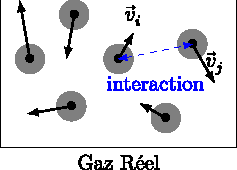
\includegraphics[width=\linewidth]{gaz_reel}
        \end{minipage}
        \begin{minipage}{0.49\linewidth}
            \centering
            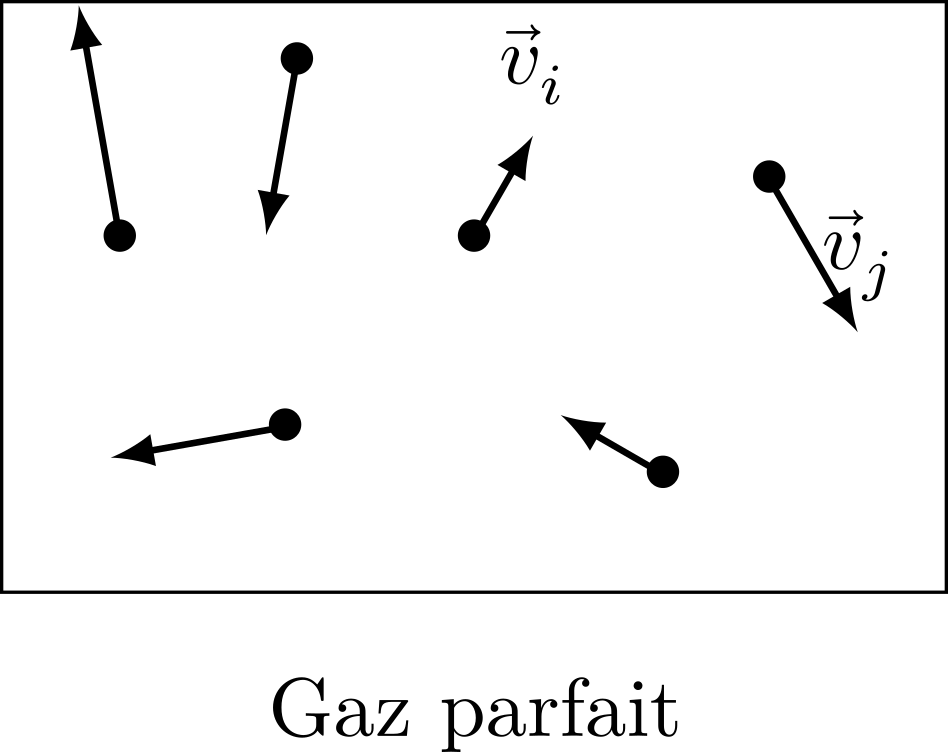
\includegraphics[width=\linewidth]{gaz_parfait}
        \end{minipage}
    \end{defi}
    \begin{loi}[label=loi:gp]{du gaz parfait}
        Lorsque la pression est assez faible ($\lesssim \SI{1}{bar}$) et à des
        températures assez élevées, les grandeurs physiques décrivant un gaz
        sont reliées par la formule
        \begin{gather*}
            \boxed{pV = nRT}
            \qavec
            \left\{
                \begin{array}{ll}
                    p & \text{en Pa }\\
                    V & \text{en m}^3\\
                    n & \text{en mol}\\
                    T & \text{en \textbf{Kelvin} (K)}
                \end{array}
            \right.\\
            \text{et }
            \boxed{R = \SI{8.314}{J.mol^{-1}.K^{-1}}}\\
            \text{est la constante des gaz parfaits}
        \end{gather*}
    \end{loi}
\end{tcbraster}
\begin{exem}[label=exem:gp, sidebyside]{application}
    On considère une seringue cylindrique de \SI{10}{cm} le long et de
    \SI{2.5}{cm} de diamètre, contenant \SI{0.250}{g} de diazote de masse
    molaire $M({\rm N}_2) = \SI{28.01}{g.mol^{-1}}$ à la
    température $T = \SI{20}{\degreeCelsius}$.
    \begin{enumerate}
        \item Calculer le volume de la seringue
        \item Calculer la quantité de matière dans la seringue
        \item Calculer la pression exercée par le diazote dans la seringue
    \end{enumerate}
    \tcblower
\end{exem}
\begin{tcbraster}[raster columns=2, raster equal height=rows]
    \begin{defi}[label=def:volmol]{volume molaire}
        Le \textbf{volume molaire} $V_m$ d'un corps est le volume occupé par
        \textbf{une mole} de gaz~:
        \[\boxed{V_m = \frac{V}{n}} \Leftrightarrow n = \frac{V}{V_m}\]
        \tcbsubtitle[before skip=\baselineskip,
        colback=green!50!black,
        colframe=green!50!black]{Unités}
        $V_m$ s'exprime en \si{m^3.mol^{-1}} ou en \si{L.mol^{-1}}
    \end{defi}
    \begin{exem}[label=exem:volmol]{volume molaire}
        Calculer le volume molaire d'un gaz parfait pour $\theta_1 =
        \SI{0}{\degreeCelsius}$ et $\theta_2 = \SI{25}{\degreeCelsius}$ avec $p
        = \SI{1013}{hPa}$.
        \tcblower
        \begin{gather*}
           T_1 = \SI{273.15}{K} \Rightarrow \DS V_m = \frac{RT}{p} =
                \SI{22.4}{L.mol^{-1}} \\
           T_2 = \SI{298.15}{K} \Rightarrow \DS V_m = \frac{RT}{p} =
                \SI{24.5}{L.mol^{-1}}
        \end{gather*}
    \end{exem}
\end{tcbraster}

\subsubsection{Pression partielle}
\begin{tcbraster}[raster columns=2, raster equal height=rows]
    \begin{defi}[label=def:ppartielle]{pression partielle}
        La \textbf{pression partielle} $P_i$ d'une espèce gazeuse $X_i$ au sein d'un
        mélange de gaz parfaits de volume $V$ et de température $T$ est égale à
        la \textbf{pression qu'aurait le système si l'espèce $X_i$ était la
        seule à occuper tout le volume}~:
        \[\boxed{P_iV = n_i RT}\]
    \end{defi}

\end{tcbraster}

\subsubsection{Loi de \textsc{Dalton}}
\begin{tcbraster}[raster columns=2, raster equal height=rows]
    \begin{loi}[label=loi:dalton]{\textsc{Dalton}}
        
    \end{loi}
\end{tcbraster}<`0`>

\end{document}
